\begin{figure}[H]
\centering
\resizebox{0.45\textwidth}{!}{
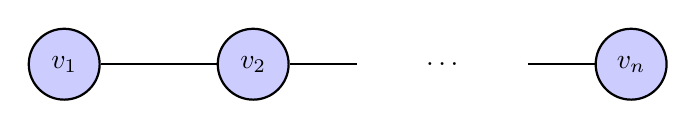
\begin{tikzpicture}[
  scale=1.2,
  vnode/.style={circle, fill=blue!20, draw=black, thick, inner sep=0pt, minimum size=0.9cm}
]

  % Posicionamiento de vértices horizontales
  \node[vnode] (v1) at (0, 0) {$v_1$};
  \node[vnode] (v2) at (2, 0) {$v_2$};
  
  % Puntos suspensivos y nodos auxiliares para conectar las aristas
  \node[draw=none, fill=none] (dots) at (4, 0) {$\dots$};
  \node[draw=none, fill=none, inner sep=0pt, minimum size=0pt] (v2_out) at (3.1, 0) {};
  \node[draw=none, fill=none, inner sep=0pt, minimum size=0pt] (vn_in) at (4.9, 0) {};

  % Vértice final
  \node[vnode] (vn) at (6, 0) {$v_n$};

  % Arista continua entre v1 y v2
  \draw[thick] (v1) -- (v2);

  % Aristas de entrada/salida hacia la elipsis
  \draw[thick] (v2) -- (v2_out);
  \draw[thick] (vn_in) -- (vn);

\end{tikzpicture}}
\caption{El grafo $P^n$}
\label{fig:camino_n}
\end{figure}
